\documentclass[aspectratio=169]{ctexbeamer}
\definecolor{urls}{RGB}{137, 180, 250}
\definecolor{link_text}{RGB}{245, 224, 220}
\hypersetup{
  colorlinks,
  linkcolor=, % This config controls the jumps inside the pdf
  urlcolor=urls,
}
\renewcommand{\UrlFont}{\ttfamily\scriptsize}

\usetheme{AnnArbor}
\usepackage[style=Mocha,accent=Rosewater]{beamercolorthemecatppuccin}

\usefonttheme{serif}
\usefonttheme{professionalfonts}

\usepackage[T1]{fontenc}
\setmainfont{LXGW WenKai}
% \setmainfont{Cascadia Code NF}
% \setsansfont{}
\setmonofont{Cascadia Code NF}
\usepackage{xeCJK}
\setCJKmainfont{LXGW WenKai}
% \setCJKmainfont{}
\setCJKmonofont{Cascadia Code NF}
\newcommand{\nerd}[1]{\texttt{#1}}
\setmonofont{Cascadia Code NF}[
  Contextuals=Alternate
]

\PassOptionsToPackage{hyphens}{url}
% \usepackage{ulem}
\usepackage{graphicx}
%\usepackage{wrapfig}
\usepackage{pifont} % Symbols used as itemize symbols
\usepackage{enumitem}
\setlist[itemize,1]{label={\small\color[RGB]{242, 205, 205}\ding{111}}}
\setlist[itemize,2]{label={\footnotesize\color[RGB]{242, 205, 205}\ding{111}}}
\usepackage{float}
\usepackage{booktabs}

\setbeamerfont{footnote}{size=\tiny}
\setbeamertemplate{footnote}{%
  \color[RGB]{108, 112, 134}%
  \insertfootnotetext%
}
\setlength{\footnotesep}{0.3\baselineskip}
\newcommand{\refnote}[1]{\footnotetext{#1}}

\usetheme{AnnArbor}

\usepackage{pifont}

\usepackage{amsmath, amssymb, amsthm}
\usepackage{listings}
\lstdefinestyle{bash-style}{
  alsoletter=-,
  keywordstyle=[2]{\color[RGB]{243, 139, 168}},
  morekeywords=[2]{sudo},
  keywordstyle=[3]{\color[RGB]{166, 227, 161}},
  morekeywords=[3]{add-apt-repository, apt-get, apt, pip},
  keywordstyle=[4]{\color[RGB]{250, 179, 135}},
  morekeywords=[4]{install},
}
\lstdefinelanguage{bash}{style=bash-style}
\lstdefinestyle{lua}{
  alsoletter=-,
  keywordstyle=[2]{\color[RGB]{137, 180, 250}},
  morekeywords=[2]{name, priority, opts, config, dependencies, submodules, main, version, init, number, boolean},
  keywordstyle=[3]{\color[RGB]{180, 190, 254}},
  morekeywords=[3]{fun, setup},
  keywordstyle=[4]{\color[RGB]{250, 179, 135}},
  morekeywords=[4]{},
}
\lstdefinestyle{path}{
  alsoletter=~,
  basicstyle={\footnotesize\ttfamily\color[RGB]{147, 153, 178}\itshape},
}
\lstset{
  language={[5.1]lua},
  style=lua,
  basicstyle=\footnotesize\ttfamily,
  breaklines=true,
  showstringspaces=false,
  breakatwhitespace=true,
  keywordstyle=\color[RGB]{245, 169, 127},
  numberstyle={\ttfamily\color[RGB]{110, 115, 141}},
  commentstyle={\color[RGB]{147, 153, 178}\itshape},
  stringstyle={\color[RGB]{166, 218, 149}},
}
% NOTE: \lstinline{} command does not support background color
\lstdefinestyle{nvim}{
  alsoletter=:,
  keywordstyle=[3]{\color[RGB]{166, 227, 161}},
  morekeywords=[3]{:Tutor, :help}, % ChkTeX 26
}

\newcommand{\TODO}[1]{\textcolor{red}{TODO\@: #1} }

% \newcommand{\link}[3][]{\href{#3}{#2}\footnote[#1]{\url{#3}}}
\newcommand{\link}[3][]{\href{#3}{#2\textsuperscript{\nerd{}}}}

\title{Neovim从入门到出门}
\subtitle{第九节：代码调试}
\author{Jacky-Lzx}
\date{\today}

\usepackage{tikz}
\titlegraphic {
  \begin{tikzpicture}[overlay,remember picture]
    \node at (-6, 4.5){
      
\includegraphics[height=1cm]{./Figures/Neovim_logo.png}
    };
    \node at (6, 4.5){
      
\includegraphics[height=1cm]{./Figures/Catppuccin_logo.png}
    };
  \end{tikzpicture}
}

\usepackage{makecell}

% ChkTeX-file 19
\begin{document}

\begin{frame}
  \titlepage
\end{frame}
\begin{frame}{大纲}
  \tableofcontents
\end{frame}
% Current section
\AtBeginSection[ ] {
  \begin{frame}{大纲}
    \tableofcontents[currentsection]
  \end{frame}
}

\section{代码调试介绍}

\begin{frame}{DAP}

  DAP\@: Debug Adapter
  Protocol，由微软提出的一种\link{调试协议}{https://microsoft.github.io/debug-adapter-protocol}，旨在为各种编程语言和调试器提供统一的调试接口

  \vspace{-1em}
  \begin{columns}[t]
    \begin{column}{0.5\linewidth}
      \small
      \begin{itemize}
        \item DAP之前：各个IDE为支持的语言编写各自的调试工具（不同的API接口）
          \begin{center}
            \begin{tikzpicture}
              \node (java) at (0,0) {
\includegraphics[height=0.5cm]{./Figures/Java_logo.pdf}};
              \node (cpp) at (1,0) {
\includegraphics[height=0.5cm]{./Figures/C++_logo.pdf}};
              \node (python) at (2,0) {
\includegraphics[height=0.5cm]{./Figures/Python_logo.png}};
              \node (idea) at (0,-1)
              {\href{www.jetbrains.com}{\includegraphics[height=0.5cm]{./Figures/IDEA_logo.pdf}}};
              \node (clion) at (1,-1)
              {\href{www.jetbrains.com}{\includegraphics[height=0.5cm]{./Figures/Clion_logo.pdf}}};
              \node (pycharm) at (2,-1)
              {\href{www.jetbrains.com}{\includegraphics[height=0.5cm]{./Figures/Pycharm_logo.pdf}}};

              \draw[<-,thick] (java) -- (idea);
              \draw[<-,thick] (cpp) -- (clion);
              \draw[<-,thick] (python) -- (pycharm);
            \end{tikzpicture}
          \end{center}
        \item 缺点：IDE与语言强绑定
      \end{itemize}
    \end{column}
    \pause

    \begin{column}{0.5\linewidth}
      \small
      \begin{itemize}
        \item DAP之后：编辑器通过DAP与各语言的调试器通讯
          \begin{center}
            \vspace{-1em}
            \begin{tikzpicture}
              \node (java) at (0,0) {
\includegraphics[height=0.5cm]{./Figures/Java_logo.pdf}};
              \node (cpp) at (1,0) {
\includegraphics[height=0.5cm]{./Figures/C++_logo.pdf}};
              \node (python) at (2,0) {
\includegraphics[height=0.5cm]{./Figures/Python_logo.png}};

              \draw (0, -1) node [draw,align=center] (java_lsp) {\tiny Java\\[-0.5em] \tiny Adapter};
              \draw (1, -1) node [draw,align=center] (cpp_lsp) {\tiny C++\\[-0.5em] \tiny Adapter};
              \draw (2, -1) node [draw,align=center] (python_lsp) {\tiny Python\\[-0.5em] \tiny Adapter};

              \node (vscode) at (0.5,-3)
              {\href{https://code.visualstudio.com/}{\includegraphics[height=0.5cm]{./Figures/Vscode_logo.pdf}}};
              \node (neovim) at (1.5,-3)
              {\href{https://neovim.io/}{
\includegraphics[height=0.5cm]{./Figures/Neovim_logo.png}}};

              \draw (1, -2) node [draw,align=center] (DAP) {\tiny DAP};

              \draw[<-,thick] (java) -- (java_lsp);
              \draw[<-,thick] (cpp) -- (cpp_lsp);
              \draw[<-,thick] (python) -- (python_lsp);

              \draw[<-,thick] (java_lsp.south) -- (DAP);
              \draw[<-,thick] (cpp_lsp.south) -- (DAP);
              \draw[<-,thick] (python_lsp.south) -- (DAP);

              \draw[<-,thick] (java_lsp.south) -- (DAP);
              \draw[<-,thick] (cpp_lsp.south) -- (DAP);
              \draw[<-,thick] (python_lsp.south) -- (DAP);

              \draw[<-,thick] (DAP) -- (neovim);
              \draw[<-,thick] (DAP) -- (vscode);
            \end{tikzpicture}
            \vspace{-1em}
          \end{center}
        \item 优点：编辑器与语言解耦
      \end{itemize}
    \end{column}
  \end{columns}

\end{frame}

\section{插件安装和配置}

\subsection{nvim-dap：代码调试器}
\begin{frame}{\link{nvim-dap}{https://github.com/mfussenegger/nvim-dap}：代码调试器}

  \begin{itemize}
    \item 插件配置：\lstinline[language={},style=path]{\~/.config/nvim/lua/plugins/dap.lua}
    \item Python调式配置：\lstinline[language={},style=path]{\~/.config/nvim/lua/plugins/languages/python.lua}
      \begin{itemize}
        \item 配置参考：\url{https://codeberg.org/mfussenegger/nvim-dap/wiki/Debug-Adapter-installation}
        \item Adapter
        \item Configuration
        \item \lstinline[language=bash]{pip install debugpy}
      \end{itemize}
  \end{itemize}
\end{frame}

\subsection{nvim-dap-view：代码调试ui}
\begin{frame}{\link{nvim-dap-view}{https://github.com/igorlfs/nvim-dap-view}：代码调试ui}
  \begin{figure}[H]
    \centering
    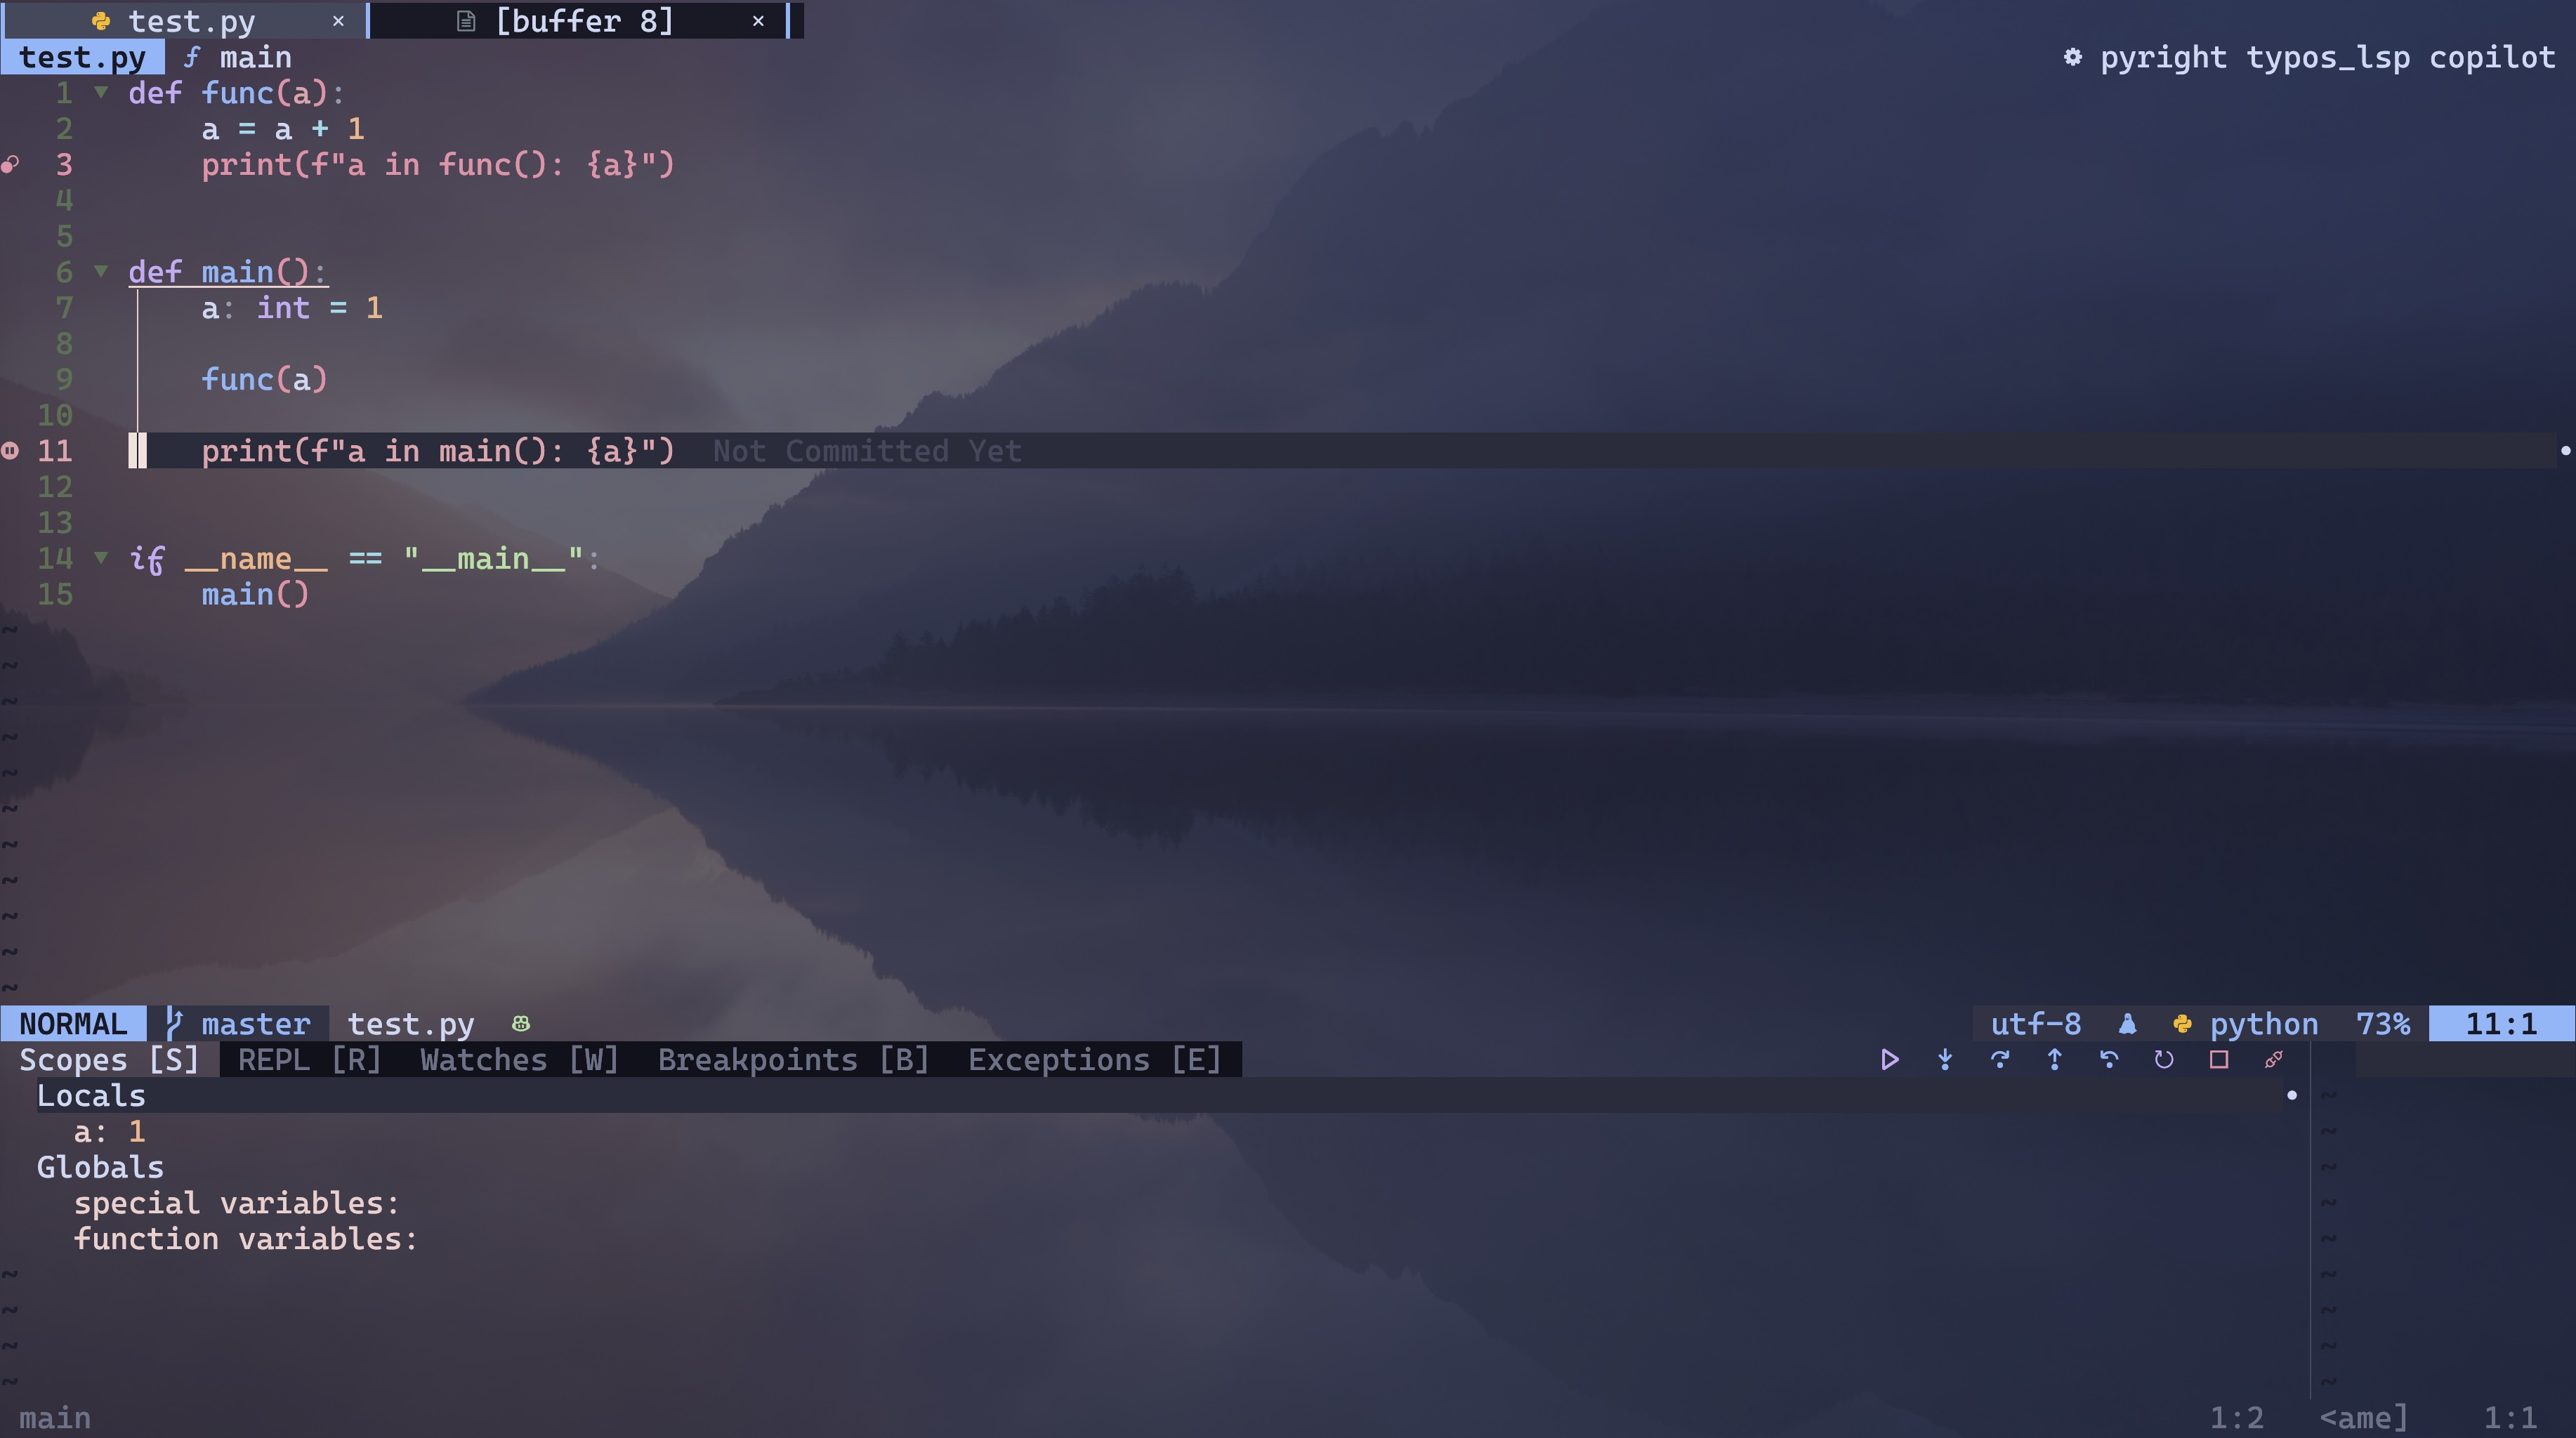
\includegraphics[width=0.65\linewidth]{./Figures/Nvim-dap-view_Finish.jpg}
  \end{figure}

  配置文件：\lstinline[language={},style=path]{\~/.config/nvim/lua/plugins/dap.lua}
\end{frame}

\begin{frame}
  \begin{itemize}
    \item 感谢：
      \begin{itemize}
        \item \link{Catppuccin}{https://catppuccin.com/} 
\includegraphics[height=10pt]{./Figures/Catppuccin_logo.png}
        \item \link{Catppuccin for beamer}{https://github.com/atticus-sullivan/beamercolortheme}
      \end{itemize}
      \vspace{0.5cm}
    \item 本教程的全部材料可以在我的Github上找到
      \begin{itemize}
        \item Slides: \url{https://github.com/Jacky-Lzx/nvim.tutorial.slides}
        \item Config: \url{https://github.com/Jacky-Lzx/nvim.tutorial.config}
      \end{itemize}
  \end{itemize}
\end{frame}

\end{document}
